\chapter{Results}\label{chapter:results}
Following providing the multivariate analysis technique described in Chapter~\ref{sec:mvas} with the simulated samples, and their systematic variations, and data, the resultant set of BDT discriminator distributions can be used to perform a measurement.

The following chapter describes the statistical methodology used to evaluate these distributions and produce a measurement of the cross section and the upper limit for the signal process and the both the expected and observed significances of this measurement.
Following a discussion of the impact that the systematic uncertainties have on the fitted results, the result presented is compared with the results made for the fully leptonic final state of tZq.

\section{Statistical Methodology}\label{sec:statisticalModel}
The Higgs Analysis Combined Limit (\combine) tool~\cite{Combine} tool, a framework based on the RooStats package~\cite{Moneta:2010pm,Schott:2012zb}, was used to perform a binned Maximum Likelihood Fit (MLF) to evaluate measurement made using the $CL_{S}$ method~\cite{CMS-NOTE-2011-005,Khachatryan:2014jba,Cowan:2010js}.

\subsection{Likelihood Model}\label{subsec:likelihoodModel}
For the signal and background processes considered in the search, the expected event yield $\lambda$ in the bin $i$ is given by equation~\ref{eq:yields1}:

\begin{equation}
\lambda_{i} = \mu s_{i} + \sum\limits_{j} b_{j} \;
\label{eq:yields1}
\end{equation}

where $s$ and $b$ are the expected number of signal and background events and $\mu$ is the signal strength modifier.
$\mu$, as given in equation~\ref{eq:signalModifier} where $\sigma_{obs}$ is the cross section observed, is used typically to parametrise the expected signal yield in lieu of the expected cross section.
The uncertainties associated with the simulated predictions of the signal and background processes are accounted for by the inclusion of nuisance parameters $\theta$, such that $s_{i} = s_{i} (\theta)$ and $b_{i} = b_{i} (\theta)$.

\begin{equation}
\mu = \frac{\sigma_{obs}}{\sigma_{s}}  \;
\label{eq:signalModifier}
\end{equation}

Assuming that the number of observed events, $n_{i}$, in any given bin will be distributed according to Poisson statistics, the probability of observing $n_{i}$ is given by equation~\ref{eq:poissonProb}.

\begin{equation}
\mathcal{P} ( n_{i} | \lambda_{i} ) = \frac{\lambda_{i}}{n_{i}!} e^{- \lambda_{i}} = \frac{ \big( \mu s_{i}(\theta) + b_{i}(\theta) \big)^{n_{i}}}{n_{i} !} e^{- \mu s_{i}(\theta) - b_{i}(\theta)}  \;
\label{eq:poissonProb}
\end{equation}

A probability density function, $\rho ( \theta | \tilde{\theta} )$ with a nominal value of $\tilde{\theta}$ for the best estimate of the nuisance, is used to describe all the sources of uncertainty for the nuisance parameters.
For the search presented in this thesis, it is assumed that each source of systematic uncertainty is either 100\% correlated or uncorrelated, thus allowing each systematic uncertainty to be incorporated into $\rho ( \theta | \tilde{\theta} )$ in a clean factorised form.
Shape uncertainties are modelled by vertically morphing the nominal shape template between between its up and down variations while the the non-prompt lepton normalisation and luminosity flat rate uncertainties are treated as log-uniform and log-normal nuisance parameters respectively~\cite{Baak:2014fta,AsymptoticFormulae}.
\combine includes the impact of the statistical uncertainty on the the aMC@NLO Z+jets sample normalisation determined in the Z+jets control region obtained as a log-normal nuisance parameter.

Therefore, the likelihood for the entire dataset can be expressed the product of the Poisson probabilities, $\mathcal{P}$, for all bins and the nuisance parameters' probability density function, as given by equation~\ref{eq:poissonLikelihood}.

\begin{equation}
\mathcal{L} ( n_{i} | \mu , \theta ) = 
\prod_{i=1}^{N} \mathcal{P} \big( n_{i} | \mu s_{i}(\theta) + b_{i}(\theta) \big) \rho ( \theta | \tilde{\theta} ) \;
\label{eq:poissonLikelihood}
\end{equation}

\subsection{$CL_{S}$ method}\label{subsec:CLsMethod}
The modified classical frequentist method, known as the $CL_{S}$ method, was used to evaluate the compatibility of data with the \emph{signal+background} (s+b) and \emph{background only} (b-only) hypotheses in terms of the siginfiance of and the limits on the signal strength measured~\cite{Cowan:2010js}.

To evaluate these hypotheses, the method constructs a test statistic, $q_{\mu}$.
The ATLAS and CMS collaborations at the LHC define $q_{\mu}$ as the log likelihood ratio for a given model with $\mu$ by equation~\ref{eq:testStatistic},

\begin{equation}
q_{\mu} =  -2 \ln \frac{ \mathcal{L}(data | \mu s , \hat{\theta_{\mu}}}{ \mathcal{L}(data | \hat{\mu} s \hat{\theta_{\mu}},  } , where 0 \leq \hat{\mu} \leq \mu \;
\label{eq:testStatistic}
\end{equation}

where $\hat{\theta_{\mu}}$ refers to the maximum likelihood estimators of $\theta$ for a given $\mu$, and 
$\hat{\mu}$ and $\hat{\theta}$ correspond to the global maximum of the likelihood. 
By definition $\hat{\mu}$ cannot take negative values as physics defines the signal rate as positive, and the constraint $\hat{\mu} < \mu$ is applied to ensure a one-sided confidence interval.

Using $q_{\mu}$, the the probability distribution functions for the \emph{s+b} and \emph{b-only} hypotheses for a given signal strength can be constructed using \emph{pseudodata} generated using toy MC for the expected outcomes of the measurement made.
For the observed outcome of the measurement, the pseudodata used for the \emph{s+b} probability distribution functions is replaced with the actual data.
From these probability distribution functions, the probability values for the s+b and b-only hypotheses can be defined as equations~\ref{eq:pmu} and~\ref{eq:1-pb}.

\begin{equation}
p_{\mu} = P ( q_{\mu} \geq  q_{\mu}^{obs} | \mu s + b ) = \int^{\infty}_{q_{\mu}^{obs}} f ( q_{\mu} | \mu , \theta_{\mu}^{obs} ) dq_{\mu} \;
\label{eq:pmu}
\end{equation}

\begin{equation}
1 - p_{b} = P ( q_{\mu} \geq  q_{\mu}^{obs} | b ) = \int^{\infty}_{q_{0}^{obs}} f ( q_{\mu} | 0 , \theta_{0}^{obs} ) dq_{\mu} \;
\label{eq:1-pb}
\end{equation}

The ratio of these probabilities are used to define $CL_{S} (\mu)$ in equation~\ref{eq:CLs}.

\begin{equation}
CL_{S} (\mu) = \frac{ p_{\mu} }{ 1 - p_{b} }\;
\label{eq:CLs}
\end{equation}

If for a given $\mu$, $CL_{S} < \alpha$, then it is said that the signal process in question is excluded with a $(1 - \alpha)$ Confidence Level (CL).
Therefore, as the 95\% CL upper limit is used in this search, the limit is determined by altering $\mu$  until $CL_{S} = 0.05$.

\subsection{Asymptotic CL$_{s}$ method}\label{subsec:asymptoticCLS}
Instead of using an ensemble of toy MC samples to generate the pseudodata, one representative dataset, known as the \emph{Asimov dataset}, was used.
This method, known as the \emph{asymptotic} CL$_{s}$ method, can be used was the number of expected events is sufficiently large and typically reduces the amount of computing time required.
The Asimov dataset is defined as being constructed such that all observable quantities are equal to their expectation values.
A full description of the asymptotic approximation to the CL$_{s}$ method is given in~\cite{Cowan:2010js}.

\section{Statistical Analysis Results}
\editComment{UPDATE BEFORE SUBMISSION AND ADD PLOTS - SPEAK TO CORIN ABOUT THIS}
For the combination of both of the final states, at the 95\% CL, the cross section for tZq production was measured to be $X^{+Y}_{-Z}$, which is within the uncertainties of the SM prediction.
This result corresponds to an observed significance of $X_{-Z}^{+Y} \sigma$ against an expected significance of $X_{-Z}^{+Y} \sigma$, which is in agreement with the SM cross section of  $0.0758^{+Y}_{-Z} \pb$.

The observed signal strengths, measured cross sections, and corresponding significances for the individual channels and their combination are shown in full in table~\ref{tab:shapetxs}.

\begin{table}[!h]
   \centering
   \caption{The observed signal strengths and corresponding cross sections for
   the individual channels and the channels combined at the 95\% CL.}
   \begin{tabular}{cccc}
       \hline
       Channel & $ee$ & $\mu\mu$ & \textbf{Combination} \\
        \hline
       Signal strength (expected) & $1_{-1.58716}^{+1.63708}$ & $X_{-0.606435}^{+0.663951}$ & $X_{-0.56704}^{+0.613355}$ \\
       Cross section (fb) & $X_{-Z}^{+Y}$ & $X_{-Z}^{+Y}$ & $X_{-Z}^{+Y}$ \\
       Significance (expected) ($\sigma$) & $0.644448_{-Z}^{+Y}$ & $1.63987_{-Z}^{+Y}$ & $1.77376_{-Z}^{+Y}$ \\
       Significance (observed) ($\sigma$) & $X_{-Z}^{+Y}$ & $X_{-Z}^{+Y}$ & $X_{-Z}^{+Y}$ \\
    \end{tabular}
   \label{tab:shapetxs}
\end{table}

At the time of writing this thesis this result is not planned to be published in its current form, as the low EXPECTED/OBSERVED significance observed is likely to be significantly improved with additional statistics.
Therefore, it is intended that a measurement on the data collected by the CMS detector during 2016 and 2017 will be performed, with the anticipation that the tZq dilepton final state can be observed.

\section{Post-Fit Impact of the Systematic Uncertainties}\label{sec:uncertainitiesImpact}
The impact of each of the sources of systematic uncertainty on the signal strength modifier $\mu$ is shown shown in figure~\ref{fig:systematicsPull}, where the left hand side of the plot illustrates the nuisance parameter residuals and the right hand side the impact of varying a nuisance parameter to its $\pm \sigma$ post-fit values has on the $\mu$.

\editComment{Discuss impact of lumi once results are in and understood}

%Given the background dominated nature of this search, it is not too surprising that the uncertainty on the luminosity %has the single largest impact on $\mu$.
%As figure~\ref{fig:systematicsPull} shows, while the maximum likelihood fit does constrain the impact of this uncertainty on the 
%

%Requiring variables constructed from the multiple jets in the final state, such as $m_{top}$, increases the sensitivity of these parameters to the resolution of the HCAL.
%
%The impact of the other experimental uncertainties are either smaller than or of the same scale as the least impactful theoretical uncertainties.
%The uncertainties in the matching of the ME and PS 
The theoretical uncertainties, while being well constrained during the 
While the impact of the theoretical uncertainties were further constrained during the MLF, each source has a an impact on the measured signal strength equal to or greater than each of the experimental uncertainties do individually (except that of the luminosity measurement).

As the  .... ISR+FSR+PS


The uncertainties associated with the Jet Energy Resolutions and Parton Distribution 
JER + PDF biggest experimental  
 
MET = small 
 
Despite the large conservative rate uncertainty ascribed to the non-prompt lepton fake shapes, 
their

given their relatively small contribution compared to other background processes and the effectiveness of the BDT in separating si, the impact 

\begin{figure}[htbp]
\begin{center}
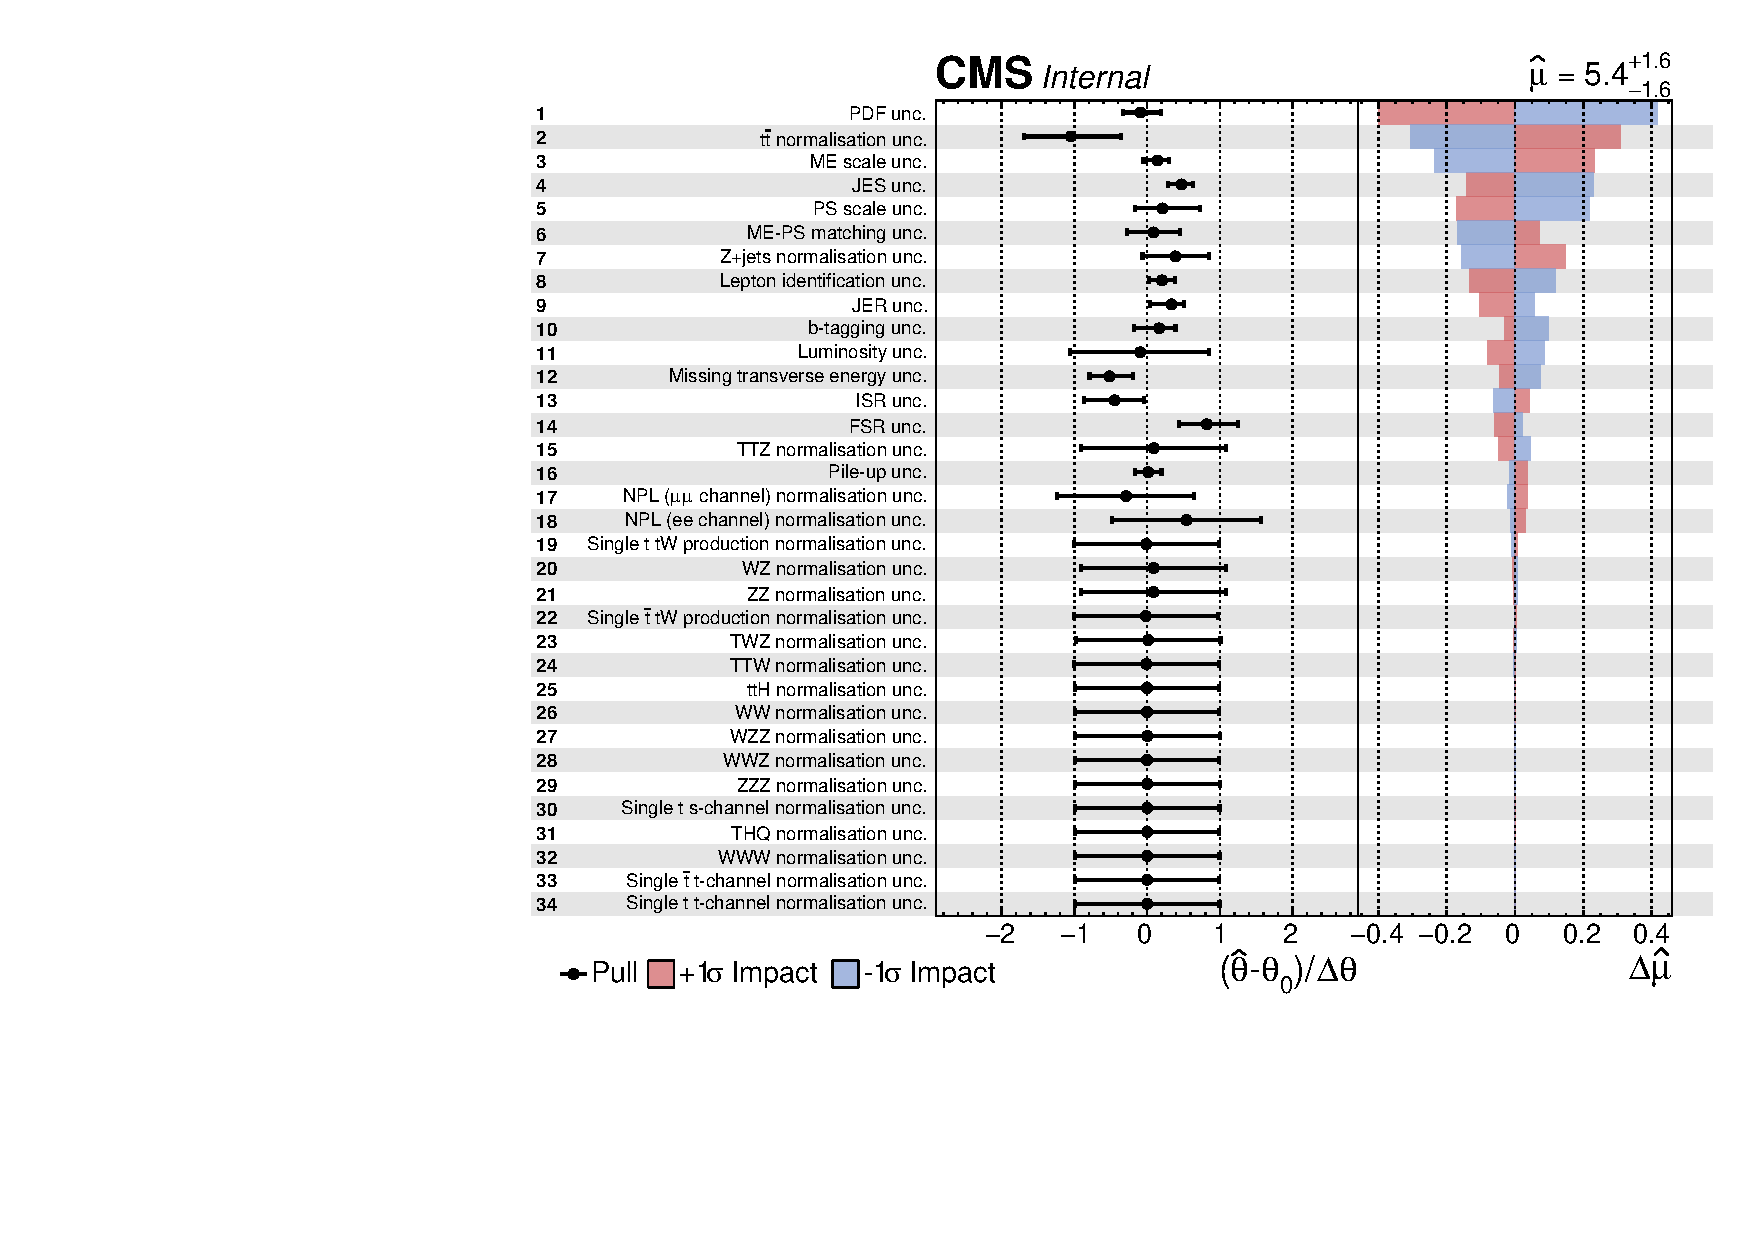
\includegraphics[width=0.97\textwidth]{figs/results/systematicsImpact.pdf}
\caption{The impact of each of the systematic uncertainties considered for the measurement made. The left hand side of the plot shows the residuals of the nuisance parameters, where $\theta$ and $\theta_{0}$ are the post-fit and pre-fit values of the nuisance parameter and $\Delta_{\theta}$ is the pre-fit uncertainty. The right hand side of the plot illustrates the shift in the signal strength parameter induced as a nuisance parameter is fixed and brought to its $\pm \sigma$ post-fit values (with the other parameters profiled as normal).}
\label{fig:systematicsPull}
\end{center}
\end{figure}

\section{Discussion of other searches for tZq at the Large Hadron Collider}
The search for the dilepton final state of a singly produced top in association with a Z boson presented in this thesis is the first one that has been undertaken at the LHC.
Therefore, while this result cannot be directly compared against any previous or competing results, its ability to observe this process can be compared against the searches performed for the fully leptonic	final state at $\sqrt{s} = 8 \TeV$ and $13 \TeV$.

The first search made for the tZq trilepton final state at $\sqrt{s} = 8 \TeV$ was made by the CMS collaboration which reported a significance of 2.9 standard deviations~\cite{Sirunyan:2017kkr}.
Following this, both the ATLAS and CMS collaborations have performed searches at $\sqrt{s} = 13 \TeV$, observing the process with reported signifiances of 4.2 and 3.7 standard deviations respectively~\cite{Aaboud:2017ylb,Sirunyan:2017nbr}.

The difference between the significances observed for the trilepton measurements and the dilepton final state measurement presented result from the different topologies of the final states.
Requiring the presence of a third lepton in the final state suppresses contributions from processes with large production cross sections, predominantly Z+jets and \ttbar, so that only such events with NPLs pass the event selection.
The modelling of the NPL background is one of main limiting factors impacting on the trileption final state measurement due to its contribution being of a comparable order of magnitude to the signal process and the large systematic uncertainty associated to the data driven estimate.
In contrast, the requirement for two well defined prompt leptons compatible with a Z boson decay significantly reduces the impact of NPL contributions despite the large uncertainties associated with them.
Conversely however, requiring two prompt leptons results permits the contributions two orders of magnitude greater than the signal process from the Z+jets and \ttbar background processes.

Given well controlled systematic uncertainties and the background dominated nature of the dilepton final state's topology limiting the ability to separate the signal process from its backgrounds, the main limiting factor for the search for tZq in the dilepton final state is the lack of sufficient statistics.
As such, the inclusion of additional data is essential if this final state is to be measured with a significance of at least 3.0 standard deviations.
In the unlikely event that a trilepton final state measurement with additional statistics is unable to measure the process with a 5.0 standard deviations significance, the combination of the updated measurements for both final states should enable the discovery of tZq.